\section{Presentazione}\label{sec:presentazione}
In questa sezione vedremo come abbiamo deciso che l'utente debba visualizzare
il nostro sito.

Come anticipato nel punto \ref{sec:struttHead}, ogni pagina può essere
visualizzata in maniera diversa a seconda del dispositivo utilizzato, vi
illustreremo quindi le scelte che abbiamo attuato nelle diverse pagine (I, II,
III Livello) in maniera tale che potessero essere visualizzate nel migliore
dei modi.

Essendo il nostro sito orientato ad un target non specifico che vuole
apprendere informazioni su diverse località, abbiamo deciso di permettere 4
diversi modi di visualizzare la pagina, applicando quindi 4 fogli di stile CSS:
\begin{itemize}
\item \textbf{Foglio di stile \texttt{layout.css}:} questo layout viene
applicato a tutti i dispositivi che visualizzano il nostro sito con più di
780px di larghezza, abbiamo però deciso di ottimizzare tale layout in maniera
che potesse essere accessibile anche a coloro che utilizzano screen-reader
\item \textbf{Foglio di stile \texttt{playout.css}:} una persona che trova
informazioni riguardo ad una località potrebbe decidere scaricare o stampare
il contenuto della nostra pagina così da poterlo guardare in un secondo tempo,
su un PDF od un foglio stampato. Questo stile serve proprio affinchè un utente
possa stampare ogni pagina del nostro sito, visualizzando al meglio le
informazioni chiave della pagina
\item \textbf{Foglio di stile \texttt{tlayout.css}:} questo foglio di stile
entra in gioco quando la pagina viene visualizzata in dispositivi con larghezza
inferiore a 780px. In tal modo il nostro sito offre una visualizzazione pulita
anche su tablet e cellulari
\item \textbf{Foglio di stile \texttt{mlayout.css}:} nel caso What To Visit
venga visualizzato su un cellulare o in una finestra con larghezza inferiore ai
480px, ecco che verrà chiamato in causa questo quarto foglio di stile, molto
simile al precedente, che permette però un eccellente visualizzazione delle
pagine di III livello anche sui cellulari. Il sito è quindi riconosciuto da
Google come \textit{Mobile-Friendly}\footnote{Il \textit{test di compatibilità
con dispositivi mobili} è stato eseguito all'indirizzo:
\texttt{https://www.google.com/webmasters/tools/mobile-friendly/}}
\end{itemize}

\subsection{I colori}\label{sec:Pres-Colore}
Prima di iniziare a guardare nel dettaglio l'aspetto grafico di ogni pagina,
vogliamo presentare quelli che sono i colori adottati nel nostro sito. In What
To Visit infatti gli utenti avranno di fronte a se delle pagine che utilizzano
pochi colori, ai quali abbiamo cercato di attribuire un significato:
\begin{itemize}
\item \textbf{Verde scuro (\#1D653C):} con questo colore, simile ad un verde
primavera scuro, abbiamo voluto indicare gli elementi non attivi ma che
possono essere attivati (come pulsanti per i commenti o i link), gli elementi
fissi della pagina (come footer ed header) oppure elementi non attivabili che
però caratterizzano una località o un collegamento (come succede per indicare
a quale categoria appartiene la località o per indicare un link che non è
stato visitato e porta in una pagina esterna al nostro sito)
\item \textbf{Verde chiaro (\#2ECC71):} Con questa via di mezzo tra un verde
primavera ed un verde smeraldo, si è deciso di indicare quegli elementi che
sono già stati attivati o che potrebbero esserlo poichè puntati dal cursore.
Un esempio possono essere i link già visitati (esterni o interni al sito),
link puntati dal cursore o ancora, i pulsanti per i commenti qualora siano
stati attivati o possano portare al cambiamento/essere frutto di un
cambiamento della pagina
\item \textbf{Grigio Scuro (\#444444):} Questo grigio scuro viene utilizzato
come colore del testo di contenuto e come colore di background per le caselle
di testo nel quale l'utente deve per l'appunto inserire informazioni o commenti
\item \textbf{Bianco (\#FFFFFF):} È presente in tutte le pagine in quanto,
colore di background del sito e della barra di ricerca presente nella
breadcrumb (Vedi punto \ref{sec:IIlev}), unica eccezione riguardante il grigio
scuro come background-color delle caselle di testo
\item \textbf{Rosso (\#E84444):} Utilizzato solamente in due casi, nelle
pagine di III livello, questo colore indica all'utente che qualcosa non va, o
che premendo un determinato puslante potrebbe cancellare i dati inseriti in
una form
\item \textbf{Grigio Chiaro (\#C9C9C9):} Questo colore viene utilizzato
solamente in un caso, quello in cui un pulsante, anche se premuto, non
cambierebbe la pagina. Questa scelta è dovuta al fatto che si vuol cercare di
far capire all'utente che quel pulsante è sostanzialmente inutile in quel
determinato momento ma che potrebbe essere utilizzato in un secondo momento
\end{itemize}

\subsection{I font}\label{sec:Pres-Font}
What To Visit è un sito che punta a catturare l'attenzione dell'utente, non
solo grazie ai suoi contenuti, ma anche grazie al suo layout.
I colori sopra descritti sono stati utilizzati per creare contrasto ed
attirare l'attenzione dell'utente in determinate aree del sito, stessa cosa è
stata fatta con i font ed il contrasto tra quelli che sono i titoli, di pagine
e paragrafi, ed il testo.

Per catturare l'attenzione del visitatore abbiamo voluto utilizzare due font
\textit{open source} importati grazie alla \textit{Google Fonts API}, parliamo
di \textbf{Open Sans Condensed} e \textbf{Roboto}, caratteri che comunque,
anche in caso di assenza, possono essere sotituiti da Arial, Helvetica e Serif
senza creare troppi problemi di visualizzazione. Ecco come sono stati
utilizzati questi due font:
\begin{itemize}
\item \textbf{Open Sans Condensed} è stato utilizzato per tutti i tag
\textbf{h1} ed i titoli di sezioni o paragrafi, questo per mettere in risalto
e catturare l'attenzione dell'utente in maniera tale che sappia a cosa si
riferisce il contenuto sottostante a tali elementi. Questo font è stato anche
utilizzato per identificare determinati link, come quelli del \textbf{Menù di
navigazione} o quelli all'interno delle liste di località;
\item \textbf{Roboto} è il font di base del sito, tutto il contenuto e la
maggior parte dei link sono scritti con questo carattere. Abbiamo voluto
utilizzare questo font in quando l'abbiamo ritenuto di facile lettura ed
ottimo nel caso di lunghi paragrafi.
\end{itemize}

\subsection{CSS3 e Parti comuni a tutte le pagine}
Durante la realizzazione del sito abbiamo cercato di creare un layout
semplice, accessibile, utilizzabile ma soprattutto visualizzabile al meglio sul
maggior numero possibile di browser. Il nostro sito limita quindi l'utilizzo
del linguaggio CSS3, un linguaggio presente ma allo stesso tempo non
fondamentale, che consente quindi un degrado elegante del sito nel caso di
mancato supporto a determinate funzioni.

CSS3 è usato in diverse parti del sito, specialmente nelle parti comuni a
tutte le pagine, già descritte nella sezione \ref{sec:struttCommon}, e
specialmente nell'ambito della visualizzazione del sito per dispositivi
mobili. Ora però vediamo come vengono visualizzati tali elementi a seconda dei
dispositivi utilizzati:

\subsubsection{Header}\label{sec:Pres-Header}
L'\textbf{Header} è un elemento presente in tutte le pagine del nostro sito
(I, II e III livello) ma viene visualizzato in maniera differente a seconda
che venga utilizzato un foglio di stile piuttosto che un altro. La differenza
principale è il modo di mostrare il nome del sito, infatti nella versione
\texttt{Screen} e \textbf{Print}, l'utente vedrà sempre comparire in
\textit{alto a sinistra} il nome del sito come una scritta, mentre nel layout
per \textbf{Dispositivi Mobili}, tramite una tecnica di
\textit{image-replacement}\footnote{Abbiamo utilizzato una sottile variante
(\texttt{text-indent}: -10em e non -9999px) del
\textit{Phark's Method} - citato da Zeldman nel 2003:
\texttt{http://www.zeldman.com/daily/0703b.shtml\#au1103}} abbiamo deciso di
far visualizzare all'utente il logo di What To Visit.
\begin{figure}[h!]
  \centering
  \begin{subfigure}[b]{0.3\textwidth}
    
\includegraphics[height=0.7cm,width=6cm]{images/pres_header.jpg}
    \caption{Header in Screen}
    \label{fig:Header-screen}
  \end{subfigure}
  \hspace{3cm}
  \begin{subfigure}[b]{0.3\textwidth}
    
\includegraphics[height=1.2cm,width=5.4cm]{images/pres_header_m.jpg}
    \caption{Header su Dispositivi Mobili}
    \label{fig:Header-mobile}
  \end{subfigure}
  \caption{Gli header di WTV}\label{fig:Display-Header}
\end{figure}

\subsubsection{Navigation menù}\label{sec:Pres-Nav}
Come accade per l'\textbf{header} anche il \textbf{menù di navigazione} è un
elemento presente in tutte le pagine del nostro sito. Questo elemento però
viene visualizzato in maniera diversa a seconda del livello della pagina e
anche del dispositivo utilizzato. Nella \textit{Homepage} infatti esso è
visualizzato nell'\textbf{header} affianco al nome del sito, mentre in tutte
le altre pagine rimane sempre nella \textit{parte alta della pagina} ma si
trova sotto alla \textbf{breadcrumb}, affianco al contenuto. Il nostro intento
però è quello di soffermarsi su come si presenta all'utente questo elemento,
quindi è importante dire che le voci di questo menù, a differenza degli altri
link, saranno di colore bianco su sfondo verde.

Nella versione \textbf{Screen} e nella \textit{homepage}, le voci del
\textbf{menù di navigazione} riprendono quelli che sono i caratteri distintivi
dei box che indicano le categorie, creando così uno stile particolare per le
pagine di I livello, cercando quindi di dare un punto di riferimento
all'utente che dovrà saper distinguere la sua posizione una volta che arriva o
ritorna nella \textit{homepage}.

La versione per \textbf{Dispositivi mobili} invece, non fa distinzione tra
pagine di \textit{I, II o III livello} e visualizza il \textbf{menù di
navigazione} solamente se l'utente attiverà il pulsante posto sempre in
\textit{alto a destra} sullo schermo del dispositivo, affianco a quello per la
\textbf{casella di ricerca}\footnote{Entrambi i pulsanti sono sempre visibili
e sono posizionati in \textit{alto a destra} grazie all'istruzione
\texttt{position: fixed}. Questi pulsanti, per cui abbiamo utilizzato la
tecnica di \textit{image-replacement} precedentemente descritta, non cambiano
all'attivazione, poichè pensiamo che l'utente capisca cosa abbia portato
all'apertura del menù e cosa dovrà premere per chiudere i box}. In questo caso
il menù apparirà in \textit{posizione fissa} coprendo il contenuto sotto ad
esso e, nel caso di menù a più livelli di profondità cercherà di rimarcare
questa gerarchia aumentando lo spessore dei bordi superiori ed inferiori delle
voci del sotto-menù.

Altre due particolarità delle voci del \textbf{menù di navigazione} sono:
\begin{itemize}
\item Il fatto che un link sia già stato visualizzato o meno, non cambia le
caratteristiche dell'ancora, questo poichè il \textbf{menù di navigazione}
serve all'utente per poter spostarsi all'interno del sito e quindi abbiamo
ritenuto non necessario che sapesse se fosse o meno già stato in una
determinata categoria o pagina secondaria;
\item La seconda caratteristica è che, nel caso il visitatore si trovi in una
\textit{pagina di II livello}, la voce che indica la posizione in cui si
trova, non sarà cliccabile, ma sopratutto verrà caratterizzata da un immagine
posta alla \textit{sinistra} di essa. Anche nel caso di \textit{pagine di III
livello}, il visitatore vedrà un immagine affianco alla voce che indica la
categoria in cui si trova, questa volta però l'ancora sarà utilizzabile.
\end{itemize}
\begin{figure}[h!]
        \centering
        \begin{subfigure}[b]{0.3\textwidth}
                
\includegraphics[height=2.63cm,width=6cm]{images/pres_nav.jpg}
                \caption{Menù di navigazione in Screen}
                \label{fig:Nav-screen}
        \end{subfigure}
        \hspace{4cm}
        \begin{subfigure}[b]{0.3\textwidth}
                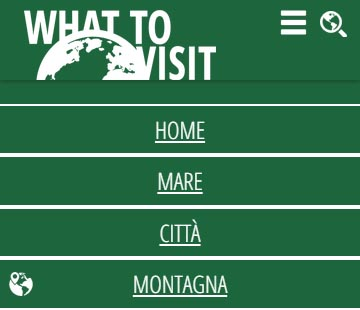
\includegraphics[height=4.65cm,width=5.4cm]{images/pres_nav_m.jpg}
                \caption{Menù di navigazione su Dispositivi mobili}
                \label{fig:Nav-mobile}
        \end{subfigure}
        \caption{I menù di navigazione di WTV}\label{fig:Display-Nav}
\end{figure}

\subsubsection{Searchbar}\label{sec:Pres-Searchbar}
La \textbf{searchbar} è un elemento presente in \textit{tutte le pagine del
sito} e, nonostante possa trovarsi in posizioni diverse, nell'\textbf{header}
per l'\textit{homepage} e nella \textbf{breadcrumb} nelle \textit{pagine di II
e III livello}, essa sarà sempre riconoscibile in quanto, oltre ad essere
l'unica casella di testo con sfondo bianco, il testo sarà verde scuro e
sopratutto il \textit{submit-botton} sarà rappresentato da una lente
d'ingrandimento, immagine spesso usata nel web per indicare la ricerca, che
verrà posta a destra della casella.

Questo elemento non viene visualizzato in maniera completamente diversa a
seconda del foglio di stile, eccezion fatta per il foglio \texttt{playout.css}
(Vedi punto \ref{sec:presentazione}) che elimina dalla stampa tale elemento in
quanto in quanto ritenuto non rilevante nel caso l'utente voglia stampare
informazioni su località o pagine secondarie.
Nelle visualizzazioni per \textbf{Screen} e per \textbf{Dispositivi mobili},
la searchbar si differenzia solamente per la posizione del
\textit{submit-botton}, posto a destra nella versione \textbf{Screen} ed a
sinistra in quella per \textbf{Dispositivi Mobili}.

\subsubsection{Footer}\label{sec:Pres-Footer}
Il \textbf{footer}, elemento con \texttt{background-color}: verde scuro, è
presente in tutte le pagine del sito. I link di questo box si comportano come
quelli del \textbf{navigation menù} (vedi \ref{sec:Pres-Nav}), sono quindi
sempre bianchi e non fanno distinzione tra ancora visitata o meno, questo
perchè servono all'utente solo come aiuto nella navigazione. Sebbene non ci
sia differenza tra \textit{visited} e \textit{unvisited}, abbiamo comunque
voluto che al passaggio del cursore ci fosse un cambiamento visivo, operato
tramite l'aumento e la diminutione del bordo inferiore.

Il \textbf{Footer} viene comunque visualizzato in maniera diversa a seconda
del foglio di stile utilizzato. La versione \textbf{Screen} e quella
\textbf{Print}, vedranno l'elemento svilupparsi orizzontalmente, occupando
tutta la larghezza della finestra, mentre nel caso di visualizzazione su
\textbf{Dispositivi mobili}, esso si svilupperà in verticale e i link puntati
cursore, si distingueranno per la presenza o meno della sottolineatura.

Un piccolo appunto sul \textbf{footer} riguarda la classe \texttt{foothome}
che, nella versione \textbf{Screen}, discrimina alcune pagine portando
l'elemento direttamente a piè pagina, utilizzando l'attributo
\texttt{position: absolute}.
\begin{figure}[h!]
        \centering
        \begin{subfigure}[b]{0.3\textwidth}
                
\includegraphics[height=0.62cm,width=6cm]{images/pres_footer.jpg}
                \caption{Footer in Screen}
                \label{fig:Footer-screen}
        \end{subfigure}
        \hspace{4cm}
        \begin{subfigure}[b]{0.3\textwidth}
                
\includegraphics[height=2.25cm,width=5.4cm]{images/pres_footer_m.jpg}
                \caption{Footer su Dispositivi mobili}
                \label{fig:Footer-mobile}
        \end{subfigure}
        \caption{I footer di WTV}\label{fig:Display-Footer}
\end{figure}

\subsection{Il layout delle pagine di I livello}\label{sec:Pres-Iliv}
Di come sono costruite le pagine, si è già parlato nella sezione
\ref{sec:struttura}, ora parliamo invece di come e cosa l'utente deve vedere
nelle pagine del nostro sito.
Nel web le cose non si vedono solo con gli occhi, ma anche con le orecchie e
magari anche con le mani; le scelte che abbiamo effettuato cercano quindi di
venire incontro alle esigenze di tutti, che utilizzino dispositivi con
dimensioni di schermo ridotte o che utilizzino screen-reader, abbiamo quindi
voluto nascondere elementi in alcune occasioni per poterli utilizzare da altre
parti, oppure abbiamo mostrato cose in un occasione ed in un altra abbiamo
fatto finta di niente.

Partiamo subito quindi parlando della nostra \textit{homepage}, l'unica pagina
di I livello e l'unica con un layout diverso dalle altre. I tre pannelli
centrali vogliono mettere il visitatore davanti ad un bivio, offrendogli però
un riscontro visivo su dove lo porterà un click su uno dei 3 box. Al
passaggio del cursore, ecco che l'immagine di sfondo aumenterà gradualmente la
sua grandezza richiamando a se l'occhio dell'utente per poi tornare
bruscamente alla sua naturale grandezza in caso il cursore vada altrove. Nel
caso in cui CSS3 non fosse supportato dal browser dell'utente, ciò non
comporterebbe disagio poiché l'immagine verrebbe istantaneamente ingrandita,
permettendo al visitatore di comprendere che sta per scegliere la categoria
sopra la quale ha fatto scorrere il mouse.

Oltre ai 3 box, cliccabili su tutta la superfice e non solo sulla parte verde
contentente il nome della categoria, nella \textit{homepage} sono presenti
\textbf{header}, contenente una \textbf{searchbar} più grande di quella delle
altre pagine, ed un \textbf{footer}, elementi già descritti in precedenza nei
paragrafi \ref{sec:Pres-Header}, \ref{sec:Pres-Searchbar} e
\ref{sec:Pres-Footer} e che, come accade per i 3 \textit{homepanel}, si
sviluppano in verticale anziché orizzontalmente.
\begin{figure}[h!]
        \centering
        \begin{subfigure}[b]{0.3\textwidth}
                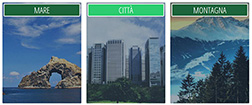
\includegraphics[height=3.7cm,width=8.9cm]{images/pres_home.jpg}
                \caption{Homepage in Screen}
                \label{fig:Home-screen}
        \end{subfigure}
        \hspace{5cm}
        \begin{subfigure}[b]{0.3\textwidth}
                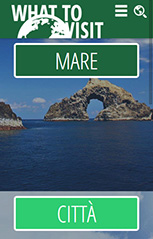
\includegraphics[height=8.43cm,width=5.4cm]{images/pres_home_m.jpg}
                \caption{Homepage su Dispositivi mobili}
                \label{fig:Home-mobile}
        \end{subfigure}
        \caption{La homepage di WTV}\label{fig:Display-Home}
\end{figure}

\subsection{Il layout delle pagine di II livello}\label{sec:Pres-IIliv}
Le pagine di secondo livello, che siano primarie o sencodarie, hanno tutte una
struttura simile così come il layout, in maniera da non creare problemi
all'utente durante la navigazione, utente che potrà però sempre contare sulla
presenza fissa di \textbf{navigation menù}, \textbf{breadcrumb},
\textbf{header} e \textbf{footer}.

Prima di passare a parlare dei due tipi di pagine di II livello, vogliamo
soffermarci sulla \textbf{breadcrumb}, quella barra che molte volte consente
all'utente di capire dove si trova e che, nonostante contenga link utili alla
navigazione, come quelli di \textbf{navigation menù} e \textbf{footer}, vede
colorare le sue ancore di verde scuro e chiaro. I colori dei link, così come
il colore di sfondo di questa barra, sono diversi da quelli del resto del sito
poichè, se per il \textit{background-color} abbiamo optato per un colore molto
simile a quello di sfondo, in quanto non abbiamo ritenuto fosse sempre
importante segnalare all'utente la posizione di questo elemento, abbiamo
voluto fare diversamente con i colori dei link visto che solitamente la
\textbf{breadcrumb}, come suggerisce il nome stesso, serve a ritrovare la
strada ed a capire dove ci si trova focalizzando così la propria attenzione su
cosa c'era prima del passo appena effettuato.

\subsubsection{Il layout delle categorie}\label{sec:Pres-IIliv-cat}
Non appena un utente entra in una delle 3 pagine riguardanti le categorie di
località, il suo occhio verrà catturato dalle immagini di tutti i luoghi
presenti in quella famiglia.

Che la pagina sia visualizzata su \textbf{Dispositivi mobili} o in versione
\textbf{Screen} non cambia, l'utente è portato a focalizzare la propria
attenzione sulla lista di località che alterna immagini del luogo al nome di
esso. Non fa molta differenza quindi se la geolocalizzazione sia attiva o
meno, in quanto è solo un'aggiunta a quello che è il vero contenuto della
pagina, non importa se essa ci fornisce anche una lista delle località più
vicine a noi, perchè ciò che conta è il contenuto, ragion per cui essa non
verrà visualizzata sui \textbf{Dispositivi mobili}.

\subsubsection{Il layout delle pagine secondarie}\label{sec:Pres-IIliv-sec}
Da una parte il \textbf{menù di navigazione} e dall'altra il contenuto, anche
nelle pagine secondarie quindi l'utente potrà concentrarsi su ciò che davvero
gli interessa, ed è proprio per questo che abbiamo deciso che tutti i link
all'interno del contenuto dovessero risaltare ancora di più: da qui la scelta
di scrivere in \textit{grassetto} tutte le porzioni di testo contenute nei tag
\textbf{a}.

Nella visualizzazione di queste pagine su \textbf{Dispositivi mobili}, non
abbiamo voluto forzare la visualizzazione portando a piè pagina il
\textbf{footer}, così come nel caso di una stampa, non abbiamo voluto inserire
elementi non necessari, rendendo così stampabili solamente \textbf{header},
la \textbf{breadcrumb}, in particolare il percorso che faciliterà l'utente nel
caso volesse cercare di nuovo la pagina sul sito, ed il contenuto.

\subsubsection{Il layout Screen e Print}\label{sec:Pres-IIliv-screenPrint}
La differenza tra layout \textbf{Screen} e quello per \textbf{Dispositivi
mobili} sta nel come viene sfruttato ed occupato orizzontalmente lo spazio a
propria disposizione.
Quando l'utente guarda la pagina di una località con una finestra di
dimensione più larga di 780px, potrà notare a sinistra il \textbf{menù di
navigazione}, in centro il contenuto ed a destra.

\subsection{Il layout delle pagine di III livello}\label{sec:Pres-IIIliv}
Il III livello di pagine è quello più importante ed è quello che più cambia il
suo modo di essere visualizzato a seconda del dispositivo utilizzato.
In tutti i casi però abbiamo deciso di rendere visualizzabili il contenuto che
descrive la località e le informazioni schematiche allegate ad essa, compresa
posizione geografica, fornita grazie alla geolocalizzazione, e link utili che
nonostante conducano l'utente fuori dal nostro sito, gli permettono di
ottenere ancora più informazioni riguardo alla località su cui si stava
informando, tutto questo contrassegnado queste ancore con appositi
accorgimenti grafici.

\subsubsection{Il layout Screen e Print}\label{sec:Pres-IIIliv-Screen}
La differenza tra layout \textbf{Screen} e quello per \textbf{Dispositivi
mobili} sta nel come viene sfruttato ed occupato orizzontalmente lo spazio a
propria disposizione.

Quando l'utente guarda la pagina di una località con una finestra di
dimensione più larga di 780px, potrà notare a \textit{sinistra} il
\textbf{menù di navigazione}, al \textit{centro} il contenuto descrittivo
della località ed a \textit{destra} noterà il box di cui si parlava in
precedenza, quello con le informazioni ed i link utili inerenti a quella
località.

Questo tipo di layout punta ad occupare la finestra in tutta la sua larghezza,
offrendo così spazio a nuove soluzioni per quanto riguarda la disposizione del
testo all'interno del box centrale. In particolar modo si è deciso di mettere
come \textit{primo elemento} un immagine significativa che presenti la
località, seguita dal suo nome ed affiancata da un box che ne identifichi la
categoria.

Successivamente inizia la parte descrittiva, divisa in paragrafi ai quali è
sempre associata un immagine. La struttura del blocco centrale ci ha permesso
quindi di poter posizionare a \textit{sinistra} un immagine ed a
\textit{destra} un paragrafo ad essa associato, creando così un effetto lista
che, se associato ad un testo non particolarmente lungo e verboso, renderà
scorrevole la lettura facendo si che il sito ne tragga vantaggio.

Una volta terminata la lettura del testo su quella determinata località, ecco
che il visitatore si troverà, nel caso supporti la funzione, di fronte alla
sezione commenti, potendo così visualizzare o postare commenti su quel luogo.
La visualizzazione dei commenti viene fatta a gruppi, evitando così che
l'utente si ritrovi da un momento all'altro a vede comparire decine e decine
di recensioni. La grafica di ogni singolo commento pone in risalto la data di
pubblicazione, inserita in un apposito span con \texttt{background-color}:
verde chiaro affiancato dal nome dell'utente che ha scritto la recensione.

\subsubsection{Il layout su Dispositivi mobili}\label{sec:Pres-IIIliv-Mobile}
A differenza di quel che accade per il layout \textbf{Screen}, la descrizione
della località non è affiancata, bensì seguita, dal box con le informazioni ed
i link utili su quel luogo. Un altra differenza riguardante la visualizzazione
delle pagine di III livello su \textbf{Dispositivi mobili}, è l'alternarsi di
testo e figure, già a partite dall'immagine di presenzazione; in questo layout
infatti troveremo prima il titolo del paragrafo, poi l'immagine e
successivamente il testo.

Sempre parlando di immagini, arriviamo a discutere della differenza
fondamentale tra il layout per cellulari e quello per dispositivi con
larghezza di schermo compresa tra i 480 ed i 780px:
\begin{itemize}
\item Nel caso di dispositivi con schermo di larghezza inferiore ai 480px,
l'immagine sarà larga il 100\% della grandezza del dispositivo;
\item Nel caso di finestre con larghezza superiore a 780px, ecco che la figura
occuperà il 60\% della larghezza della finestra, questo accade sia per le
immagini dei paragrafi, sia per quelle delle liste di definizioni. Questa
distinzione è atta a far si che l'utente possa comunque godere delle immagini
messe a sua disposizione, perchè trattandosi di un sito che ha lo scopo di
introdurre al visitatore nuove località, ecco che un minimo di qualità, e
purtroppo anche di peso, è più che dovuta.
\end{itemize}

\subsection{Considerazioni finali sui fogli di stile applicati}\label{sec:Pres-CSSValid}
All'interno di ogni pagina, in \textit{basso a destra}, troverete un immagine
che indica che il nostro sito utilizza CSS valido, ma sopratutto ci teniamo a
sottolineare che abbiamo cercato di non abusare di tecnologie, quali CSS3, non
supportate da tutti i browser, creando quindi dei meccanismi che potessero in
ogni caso portare l'utente a vivere al meglio l'esperienza What To Visit.

Terminiamo questa sezione parlando quindi di come abbiamo voluto nascondere
agli occhi di molti alcuni elementi, quali alcune label che quindi non saranno
visibili all'occhio umano, o di come abbiamo cercato di nasconderne altri a
tutti, come accaduto nel caso di layout \textbf{Screen} quando abbiamo
utilizzato la caratteristica \texttt{display: none} per nascondere
completamente il form contenente i \textit{trigger} utilizzati successivamente
nei layout per \textbf{Dispositivi mobili}.
